\documentclass{standalone}
\usepackage{balloonspectacular}

\begin{document}

\begin{tikzpicture}[x=1in, y=1in]
\path[fill=white] (-46.25, -11.5) rectangle (2.25, 15.5);

%\path[draw, ultra thick, rounded corners=3mm, fill=YellowGreen!50] (-46.25, -2.75) rectangle (2.25, 15.5);

\node at (-22, 6.375) {\includegraphics[height=18.25in]{Images/play_area_background.png}};

\foreach \x in {0, -4,-8,...,-44}
 \foreach \y in {0, 4.25, ..., 12.75}
 {
	\node[cardposition] at (\x,\y) {};
	\node[cardposition, white, dashed] at (\x,\y) {};
 }

\foreach \x/\i in {-44/1, -40/2, -36/3, -32/4, -28/5, -24/6, -20/7, -16/8, -12/9, -8/10, -4/11, 0/12}
	\node[inner sep = 2cm] at (\x, 17) {{\setmainfont[Scale=5.0]{Titan One}\Huge \i}};

\foreach \x in {0, -4, ..., -44}
{
  \node[cardposition, rotate=90] at (\x, -6) {};
  \node[cardposition, white, dashed, rotate=90] at (\x, -6) {};
}

\foreach \x in {0, -4, -8, -12} {
	\node[truckcard] at (\x, -6) {\includegraphics[width=3.25in]{Images/truck_b.png}};
%	\node[cardposition] at (\x, -5.5) {};
}


\foreach \x in {-5, -5.25, ..., -6}
	\node[ballooncard, rotate=90] at (\x, -9.25) {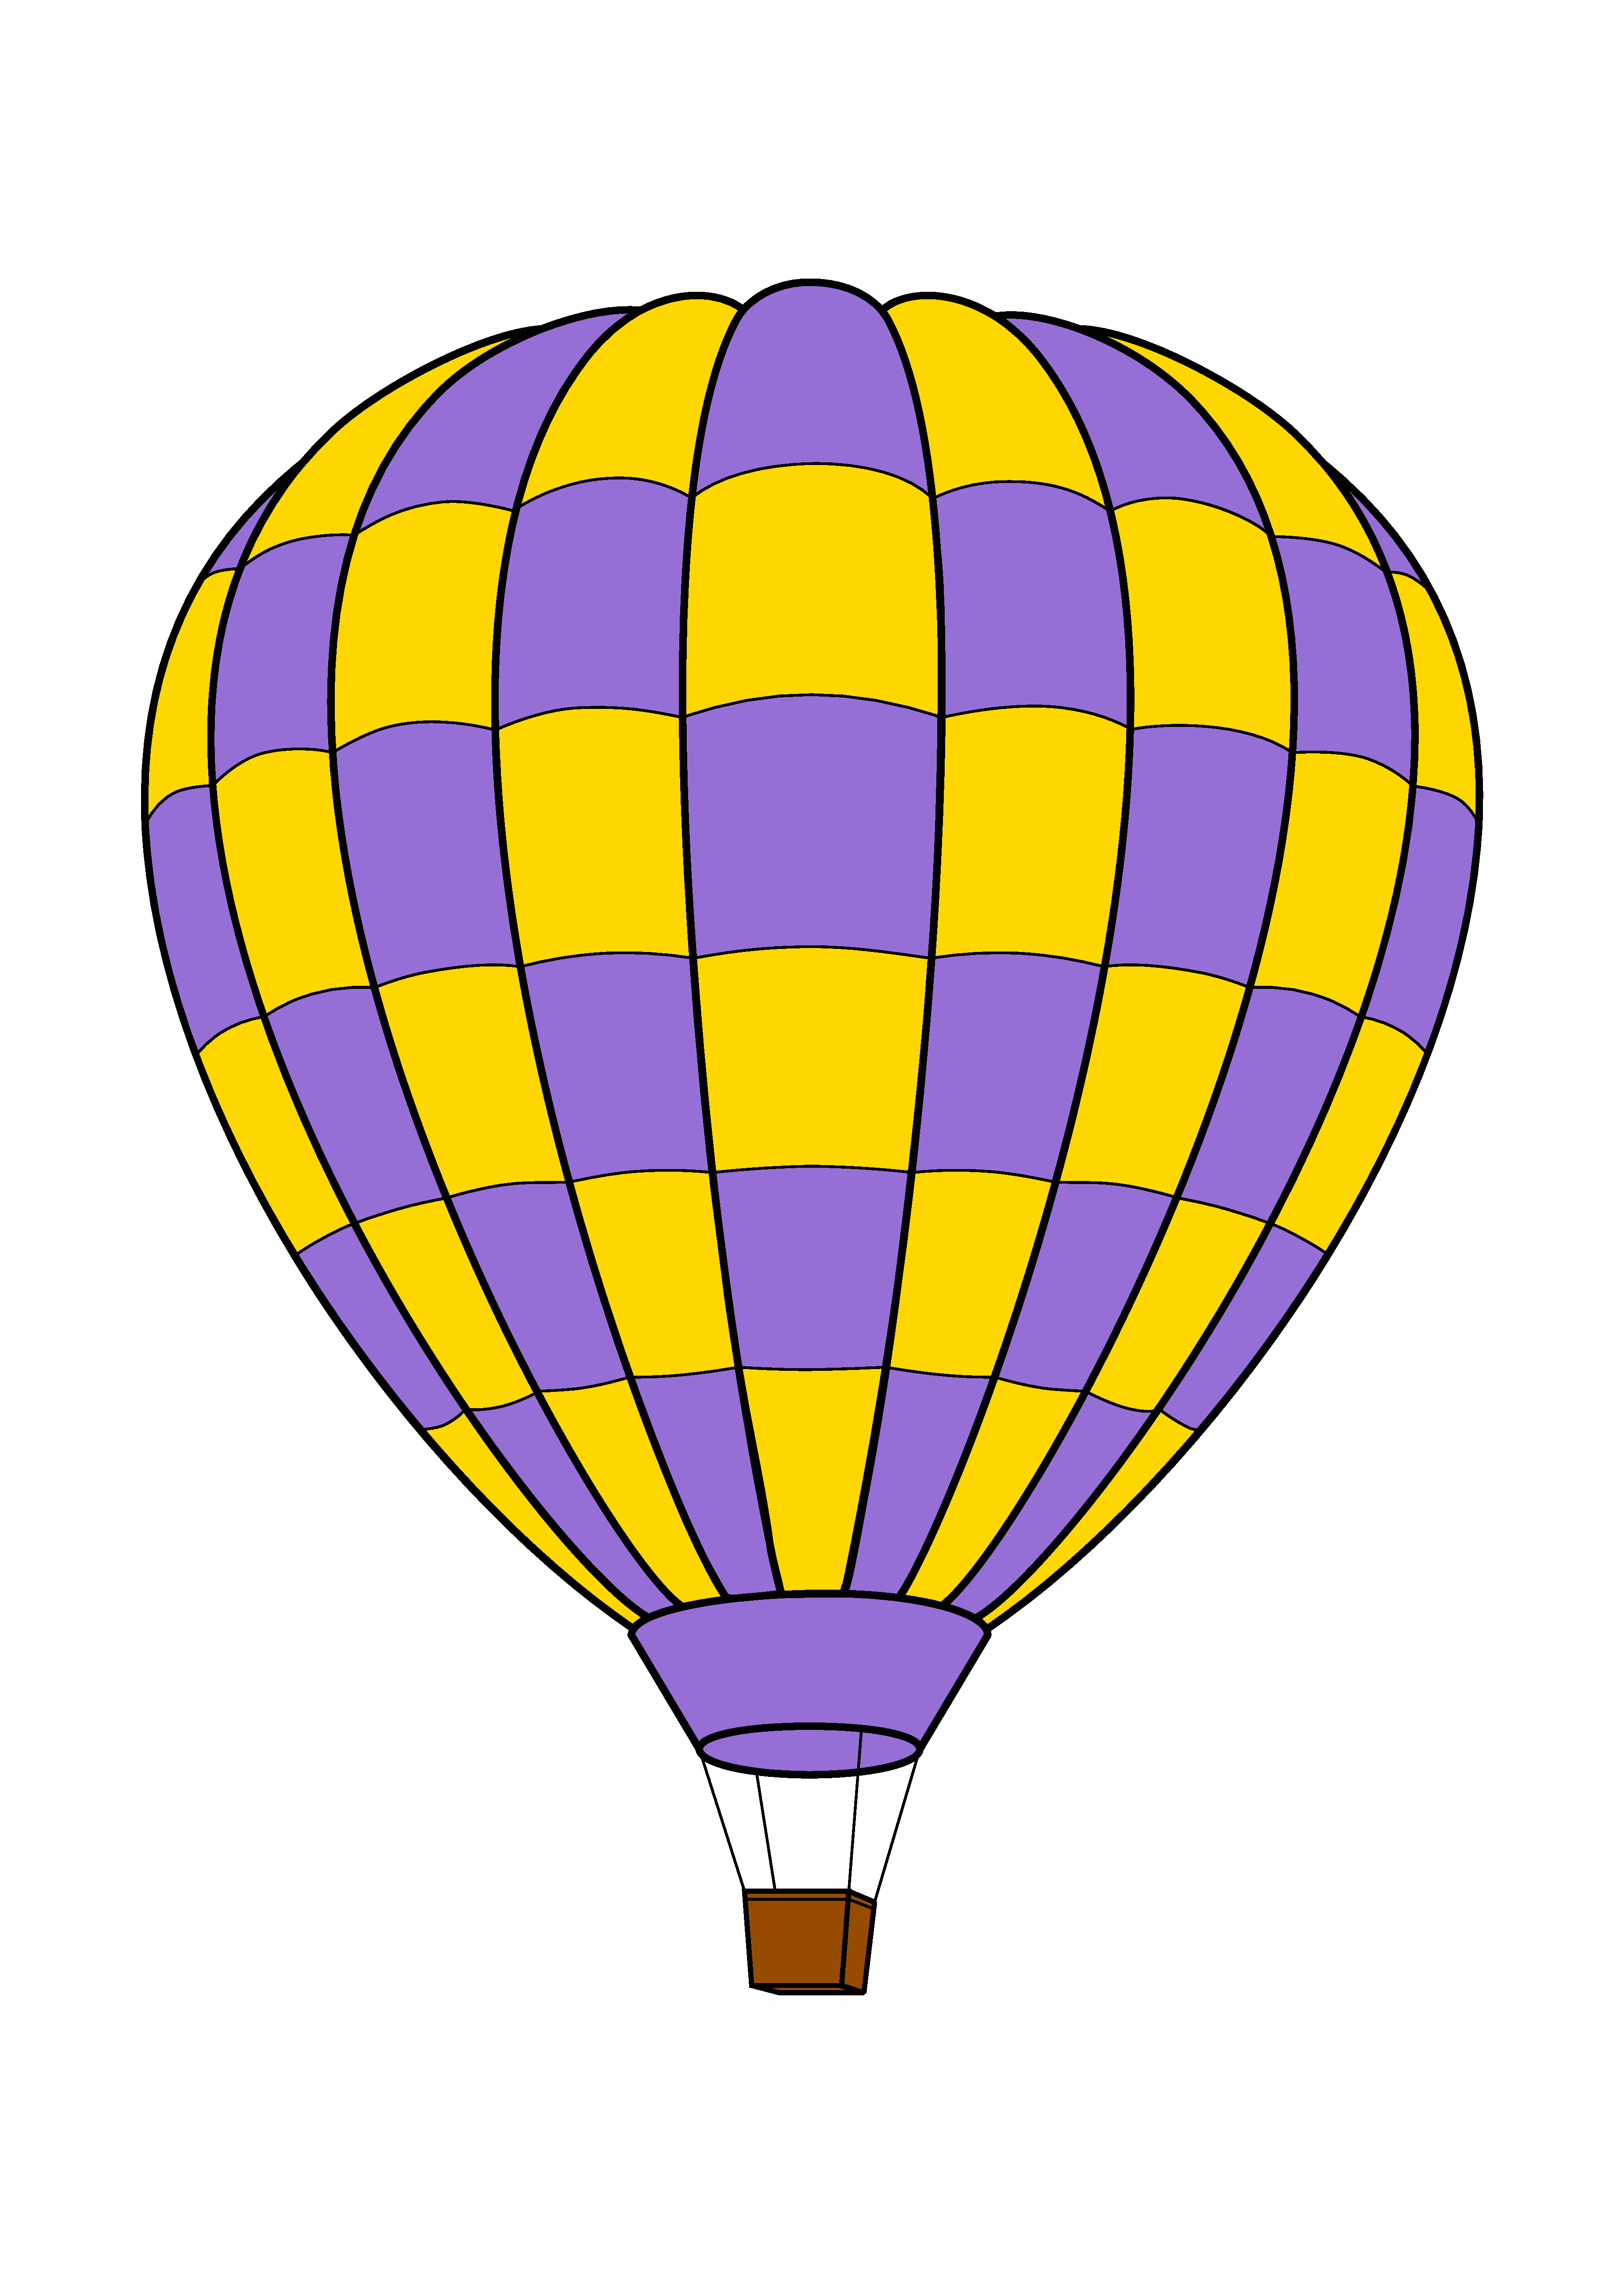
\includegraphics[height=3.25in]{Images/grid_py.png}};
	
%	\node[inner sep=1.5in] at (-22, 21) {{\setmainfont[Scale=12.0]{Oi}\Huge Aloft}};

\end{tikzpicture}

\end{document}
